\documentclass{ximera}

\graphicspath{{./auto_generated_text/Week1CoordinateSystems/graphics/}{./graphics/}}

\title{Spherical Coordinates}
\begin{document}
\begin{abstract}
\end{abstract}
\maketitle

In this activity, we introduce spherical coordinates, a new coordinate system on $\mathbb{R}^3$. We also discuss how to convert between spherical and Cartesian coordinates.

\section{Spherical Coordinates}

We've seen how to express points in $\mathbb{R}^3$ using Cartesian coordinates and using cylindrical coordinates. We'll now introduce a new coordinate system, called \emph{spherical coordinates}.

Given a point $P$ in $\mathbb{R}^3$, imagine drawing a line segment from the origin to $P$. In spherical coordinates, we write $P$ as $(\rho, \theta, \phi)$. Here, $\rho$ is the length of the segment (also the distance between $P$ and the origin). The second coordinate, $\theta$, is angle between the positive $x$-axis and the projection of the segment onto the $xy$-plane. The third coordinate, $\phi$, is the angle between the segment and the positive $z$-axis.

\begin{image}
\begin{tikzpicture}
\node[inner sep=0pt] (russell) at (0,0)
    {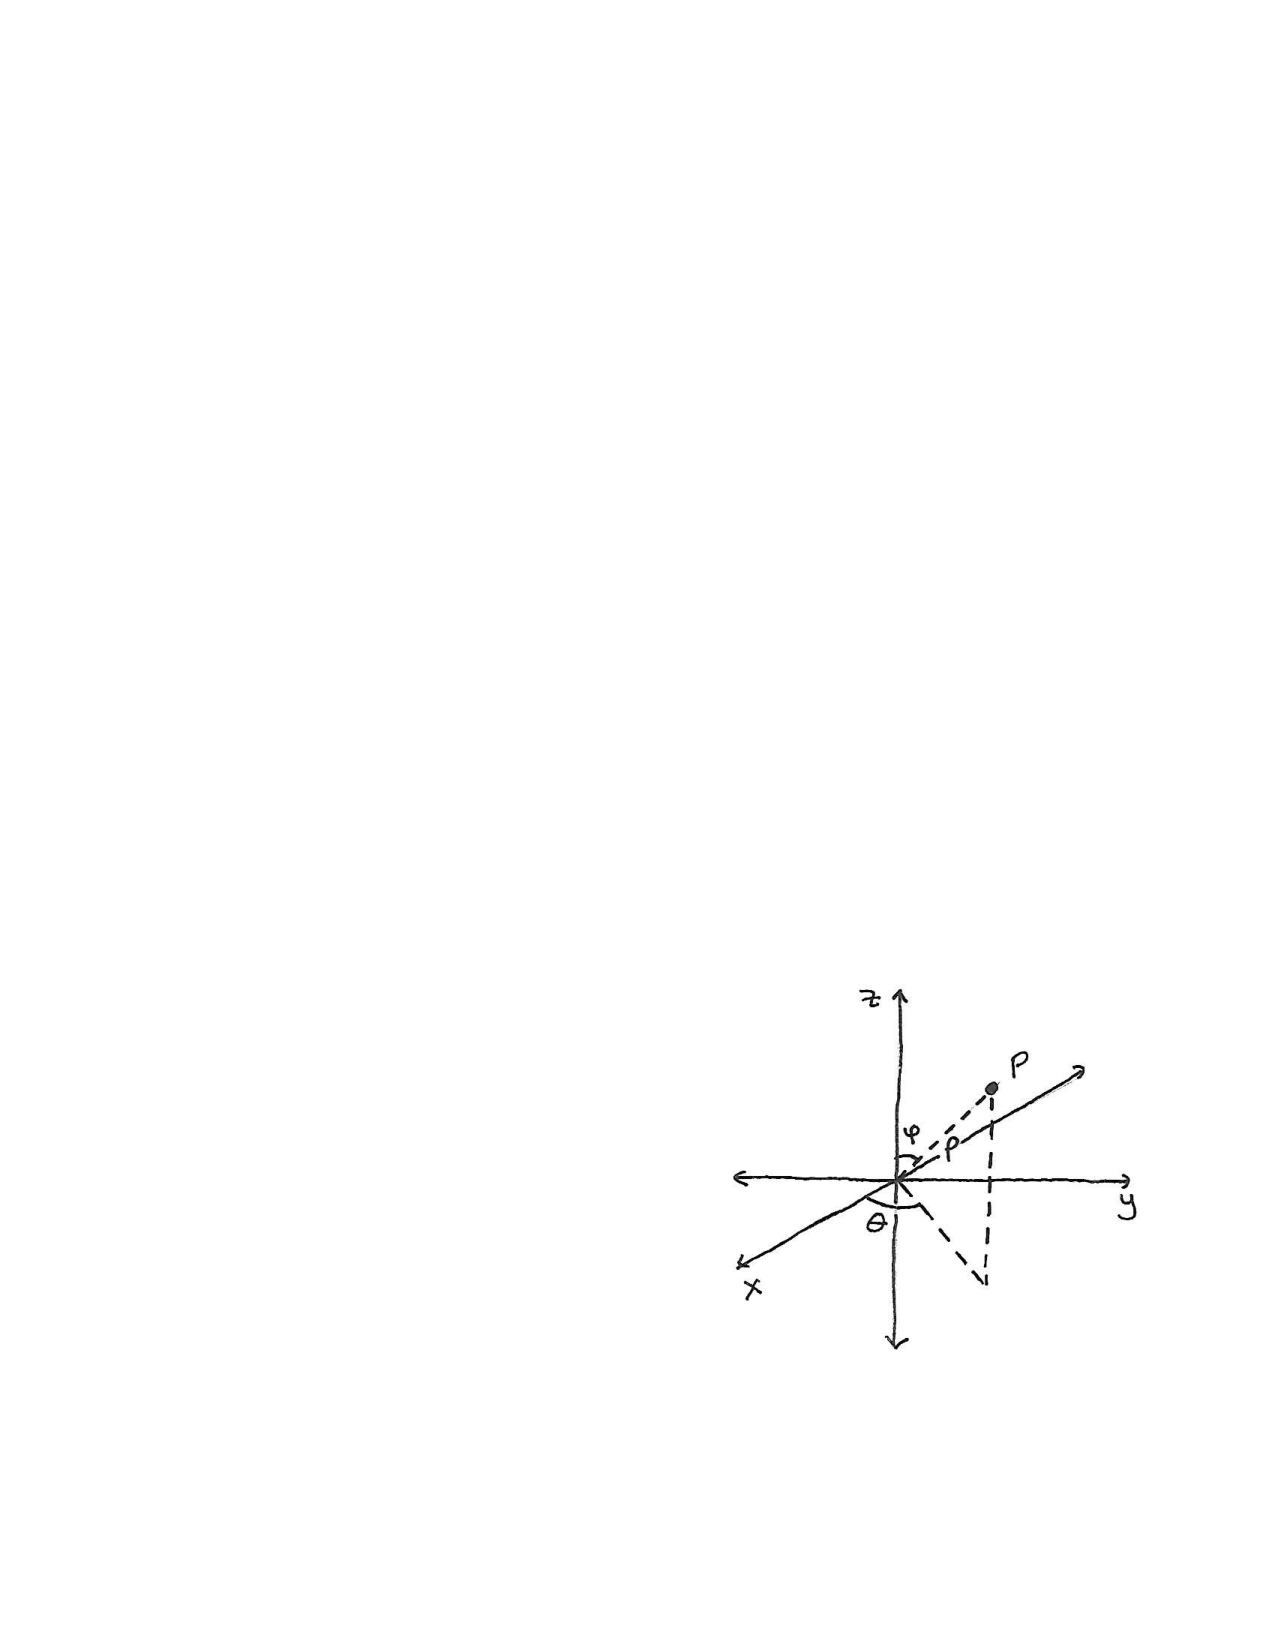
\includegraphics{spherical}};
\end{tikzpicture}
\end{image}

\begin{example}
We'll write the point $P$ in spherical coordinates, where $P$ is given by $(x,y,z) = (0,1,1)$ in Cartesian coordinates.

\begin{image}
\begin{tikzpicture}
\node[inner sep=0pt] (russell) at (0,0)
    {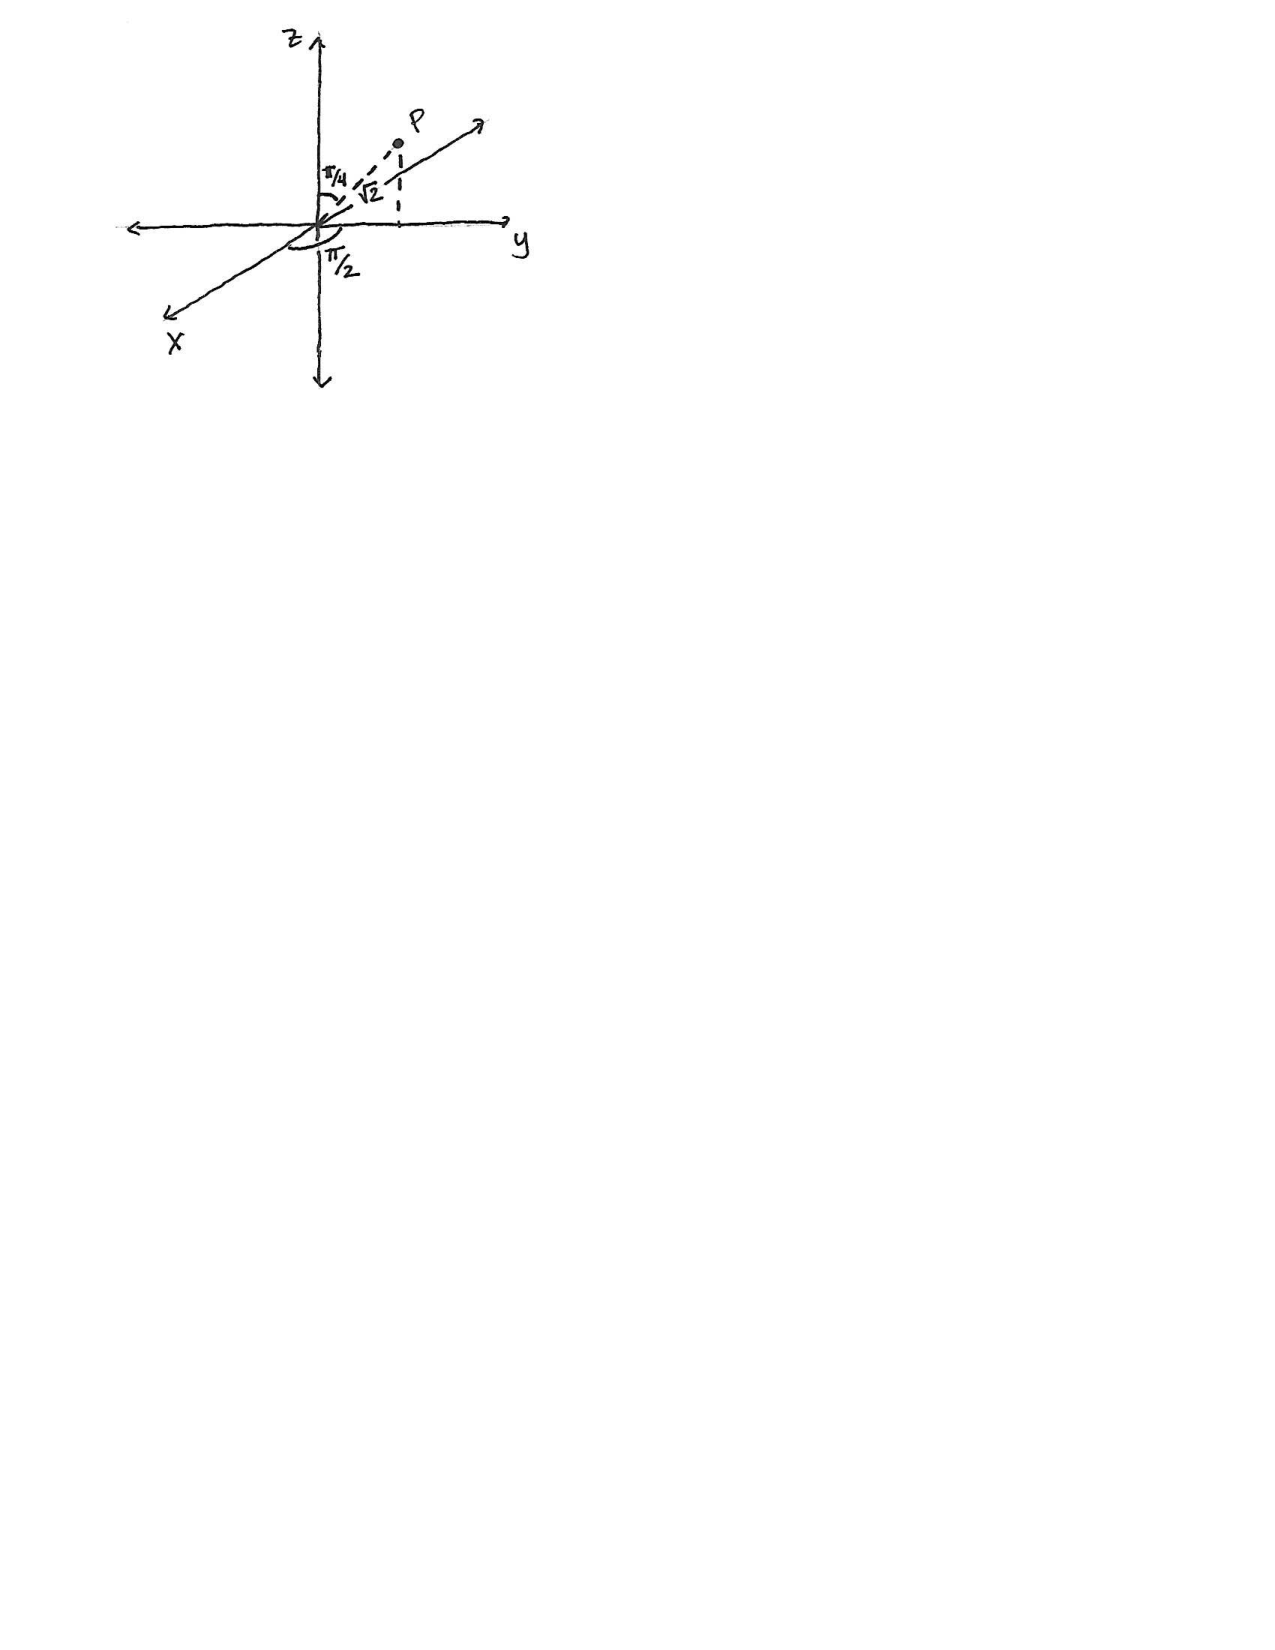
\includegraphics{011}};
\end{tikzpicture}
\end{image}

The distance between $P$ and the origin is
\[
\sqrt{0^2 + 1^2 + 1^2} = \answer{\sqrt{2}},
\]
so $\rho = \answer{\sqrt{2}}$.

The angle between the positive $x$-axis and the projection of $P$ onto the $xy$-plane is $\answer{\pi/2}$ (in radians), so $\theta = \answer{\pi/2}$.

The angle between $P$ and the positive $z$-axis is $\answer{\pi/4}$ (in radians), so $\phi = \answer{\pi/4}$.

Thus we can write $P$ in spherical coordinates as $\answer{(\sqrt{2}, \pi/2,\pi/4)}$.

\end{example}

Although we will be consistent with our definitions of $\theta$ and $\phi$ as above, it's important to know that some people reverse the roles of $\theta$ and $\phi$. This is particularly common among physicists.

\section{Uniqueness}

As with polar and cylindrical coordinates, there are issues of uniqueness with spherical coordinates that we do not encounter in Cartesian coordinates.

Let's take for the example the point $(x,y,z) = (0,1,1)$, written in Cartesian coordinates. We've seen the canonical way to write this point in spherical coordinates, as $(\sqrt{2}, \pi/2, \pi/4)$. However, we could also write this as $(\sqrt{2}, 5\pi/2, \pi/4)$, $(\sqrt{2}, -3\pi/2, \pi/4)$, or even $(-\sqrt{2}, 3\pi/2, 5\pi/4)$.

Because of this issue, we'll commonly use the restrictions
\begin{align*}
0\leq &\rho\\
0\leq &\theta<2\pi\\
0\leq &\phi\leq\pi
\end{align*}
when working with spherical coordinates in order to improve the uniqueness situation. Unfortunately, there are still multiple ways to represent the origin in spherical coordinates.

\begin{problem}
Which of the following represent the origin in spherical coordinates? Select all that apply.
\begin{selectAll}
\choice[correct]{$(0,0,0)$}
\choice[correct]{$(0,\pi/2,0)$}
\choice[correct]{$(0,0,\pi/4)$}
\choice[correct]{$(0,\pi/2,\pi/4)$}
\end{selectAll}
\end{problem}

You may use the following applet to experiment with how the different coordinates change a point written in spherical coordinates.

\href{https://mathinsight.org/spherical_coordinates}{MATH INSIGHT APPLET}

\section{Constant-Coordinate Surfaces}

As we did with cylindrical coordinates, we'll see what happens when we set each of the coordinates to be constant.

Consider the set of points $(\rho, \theta, \phi)$, where $\rho = C$ is constant. This means that the distance between the origin and any such point is $C$. Varying the angles $\theta$ and $\phi$ gives us all such points, which make a sphere of radius $C$.

\begin{image}
\begin{tikzpicture}
\node[inner sep=0pt] (russell) at (0,0)
    {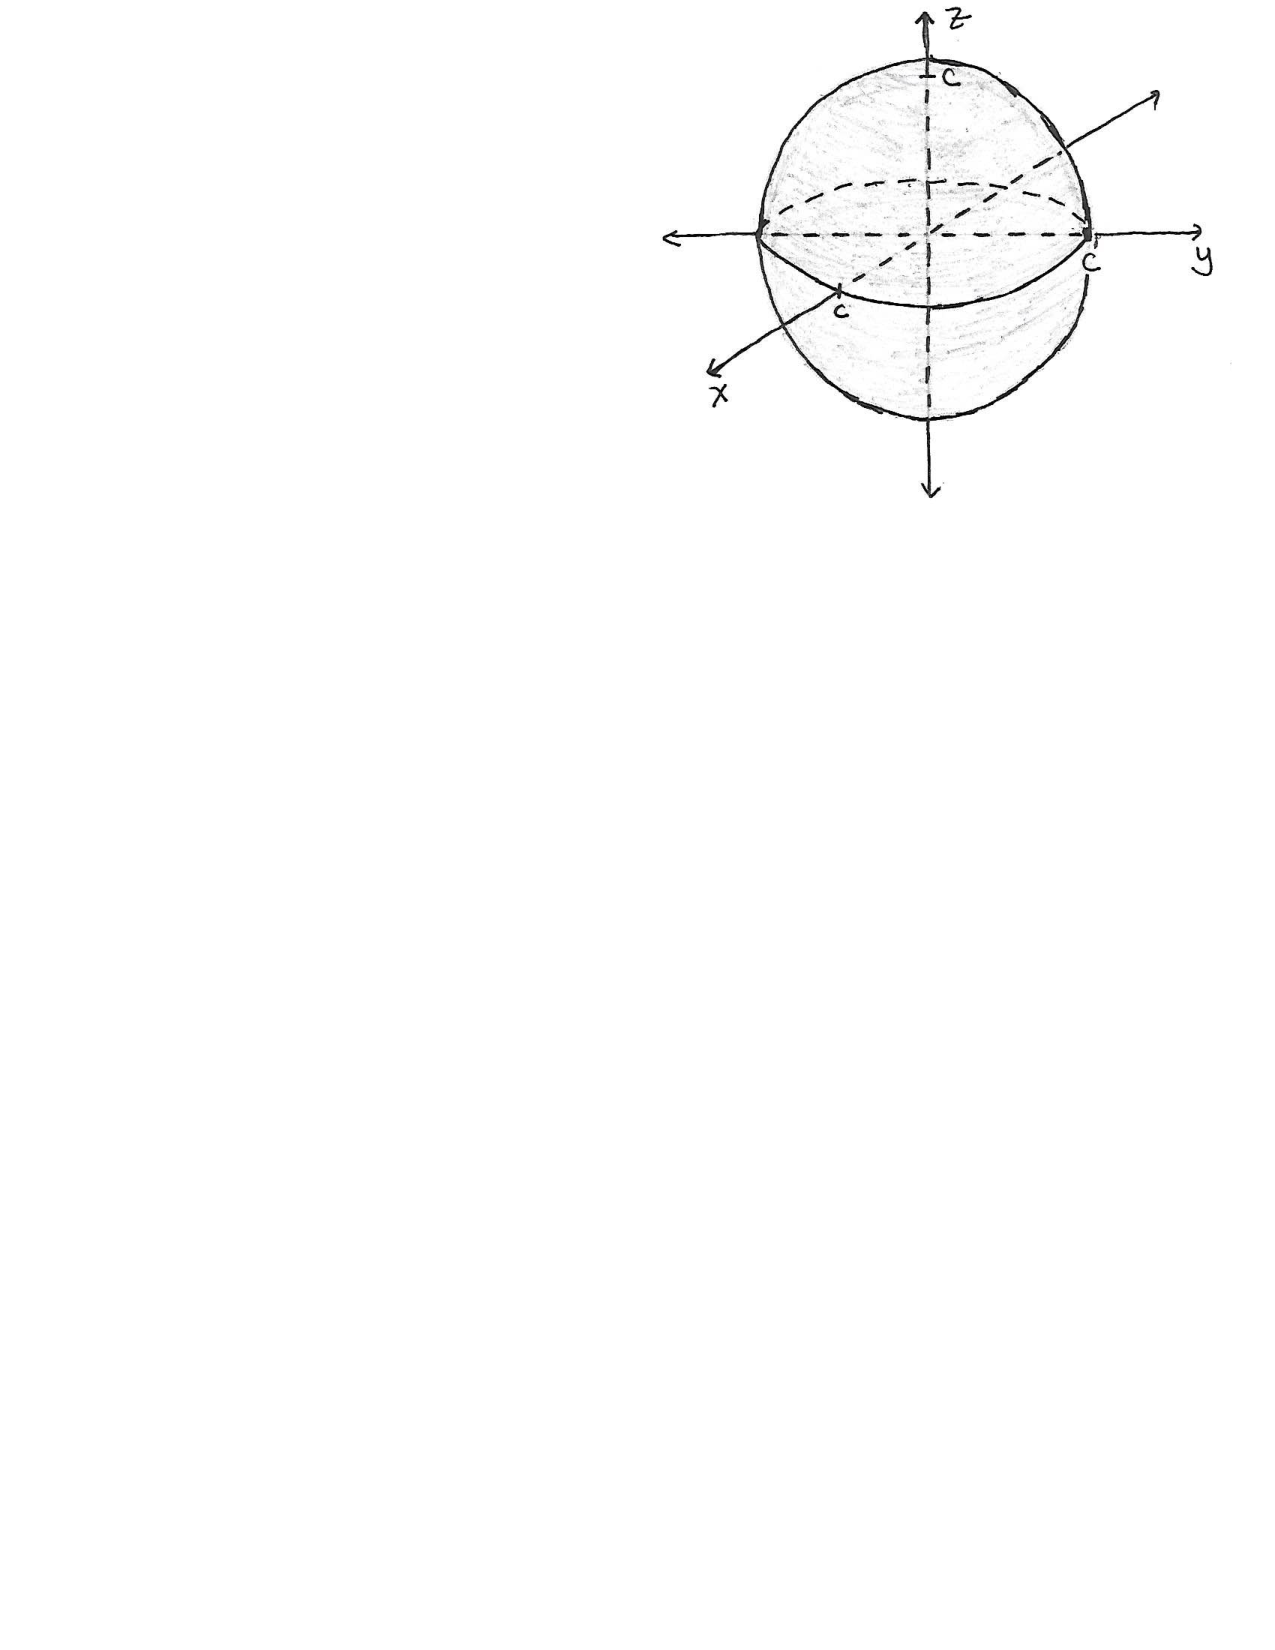
\includegraphics{rho_constant}};
\end{tikzpicture}
\end{image}

Now, consider the set of points $(\rho, \theta, \phi)$, where $\theta = C$ is constant. This means that the projection of any such point onto the $xy$-plane will make an angle $C$ with the positive $x$-axis. Varying $\rho$ gives us points at various distances from the origin, and varying $\phi$ gives us points making various angles with the positive $z$-axis. With the restrictions $\rho\geq 0$ and $0\leq \phi\leq\pi$, we obtain a half plane, as below.

\begin{image}
\begin{tikzpicture}
\node[inner sep=0pt] (russell) at (0,0)
    {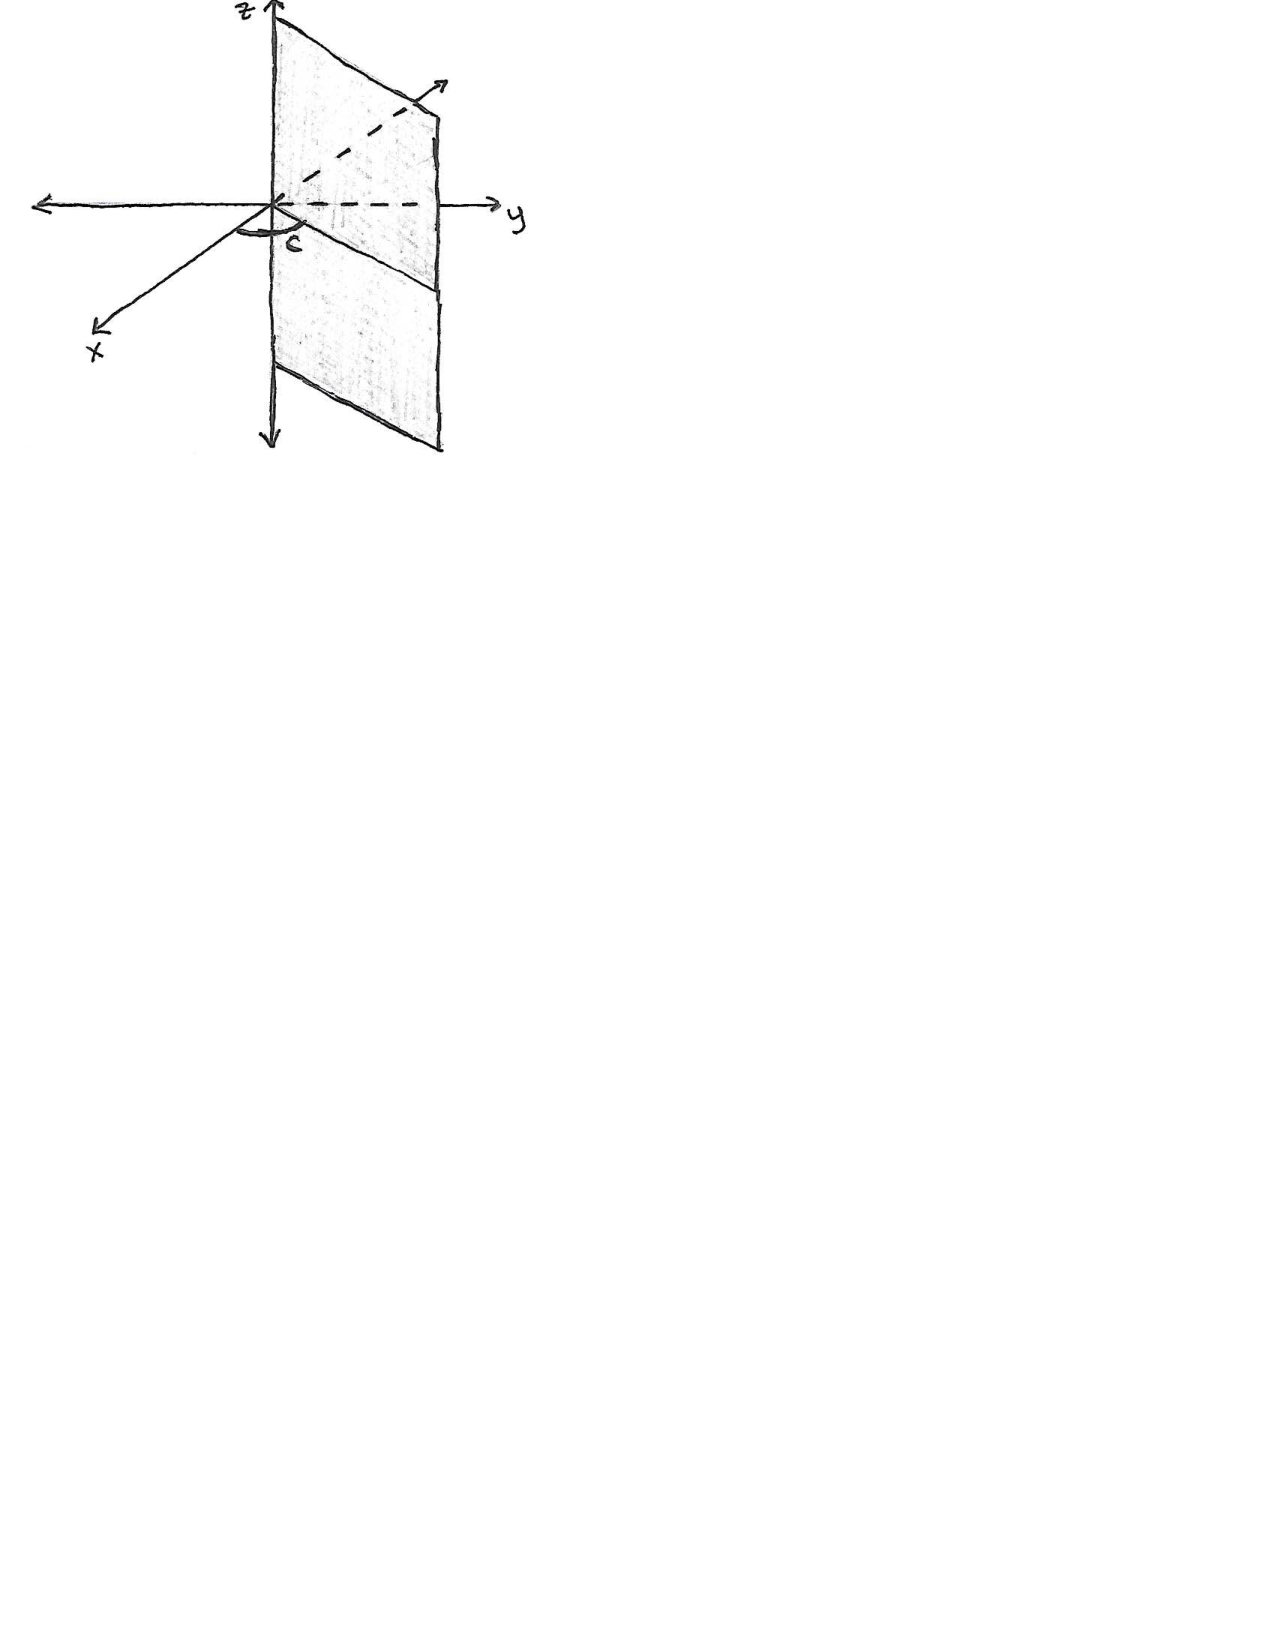
\includegraphics{theta_constant}};
\end{tikzpicture}
\end{image}

Notice that if we relaxed the restrictions on $\rho$ and $\phi$, we could obtain the entire plane.

Finally, we consider the set of points $(\rho, \theta, \phi)$, where $\phi = C$ is constant. This means that every such point has an angle $C$ with the positive $z$-axis. Varying $\rho$ and $\theta$, with the restriction $\rho\geq 0$, we get the surfaces below, depending on if $C<\pi/2$, $C=pi/2$, or $C>pi/2$.

\begin{image}
\begin{tikzpicture}
\node[inner sep=0pt] (russell) at (0,0)
    {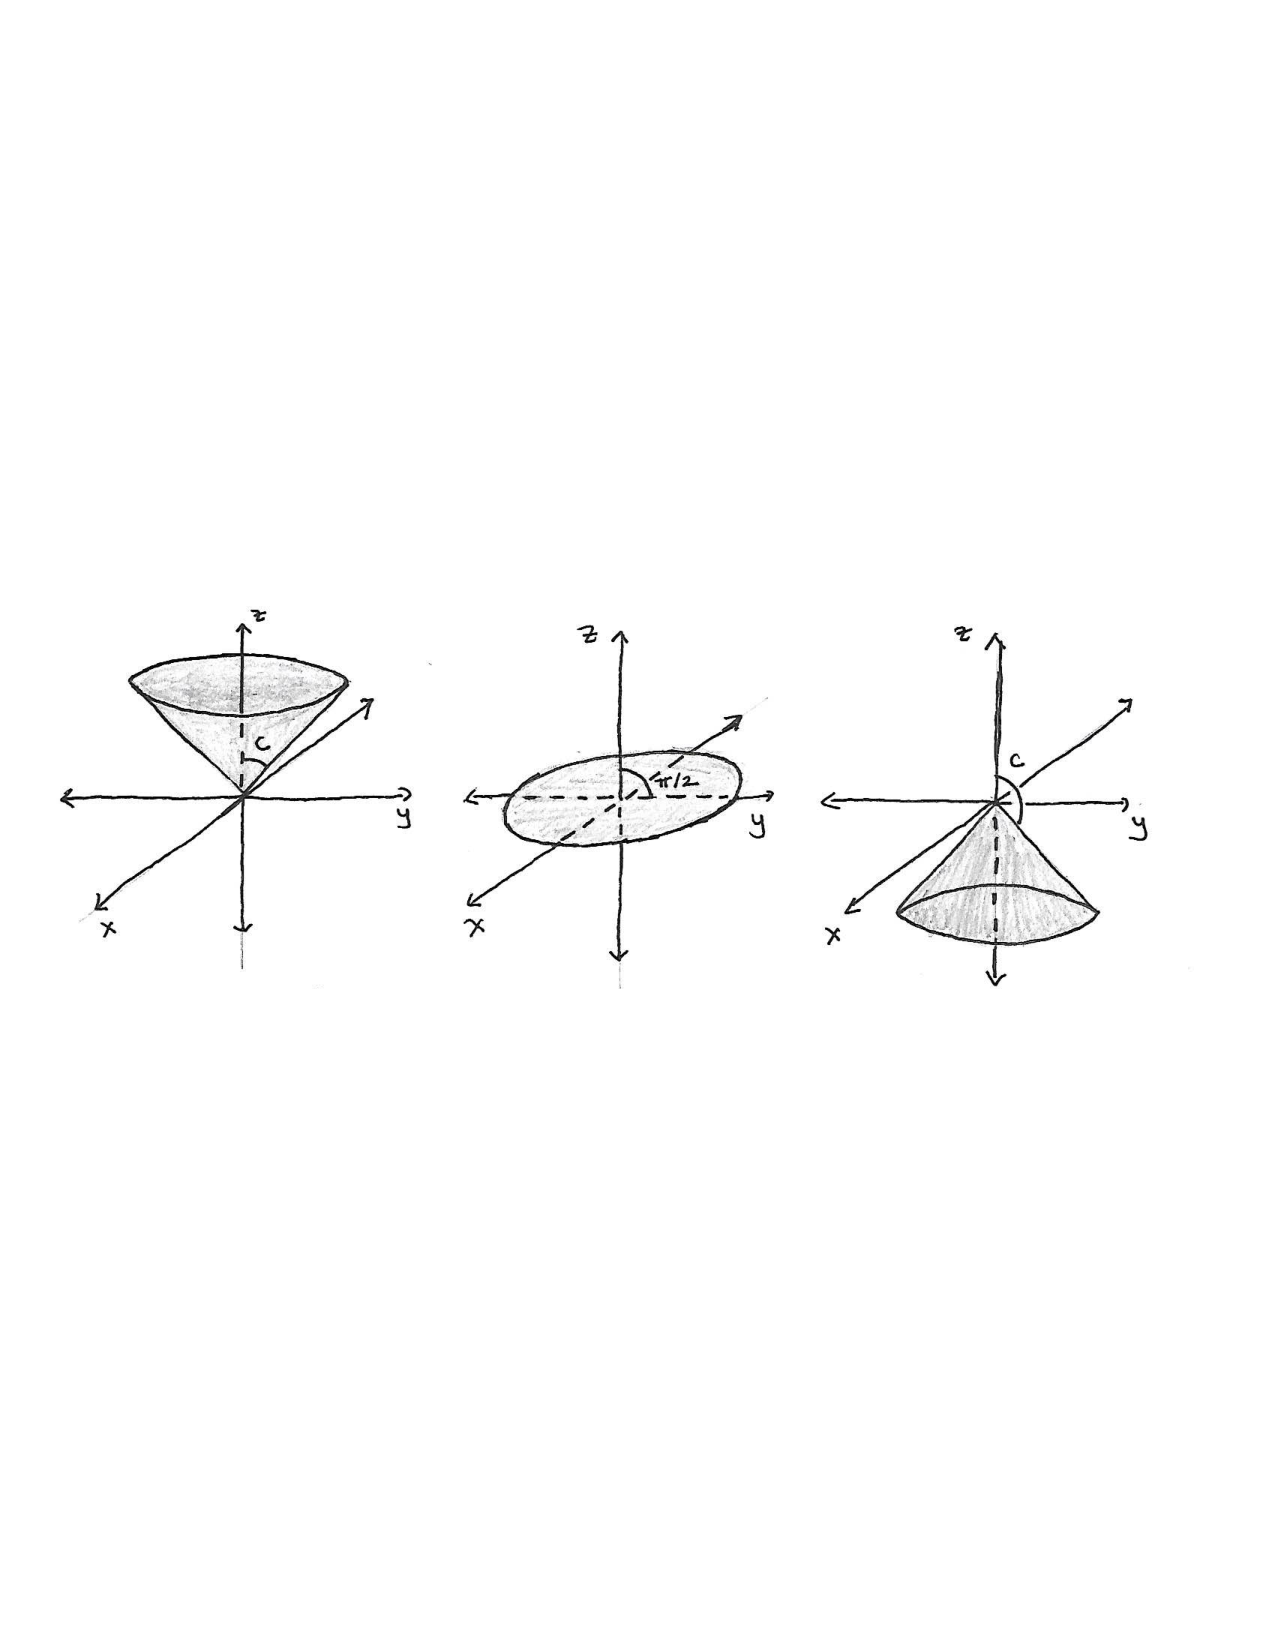
\includegraphics{phi_constant}};
\end{tikzpicture}
\end{image}

Looking at the surfaces when $C>\pi/2$ or $C<\pi/2$, we would commonly call these surfaces ``cones.'' However, in most mathematics, ``cone'' is more commonly used to describe the surface below, which you might call a double cone.

\begin{image}
\begin{tikzpicture}
\node[inner sep=0pt] (russell) at (0,0)
    {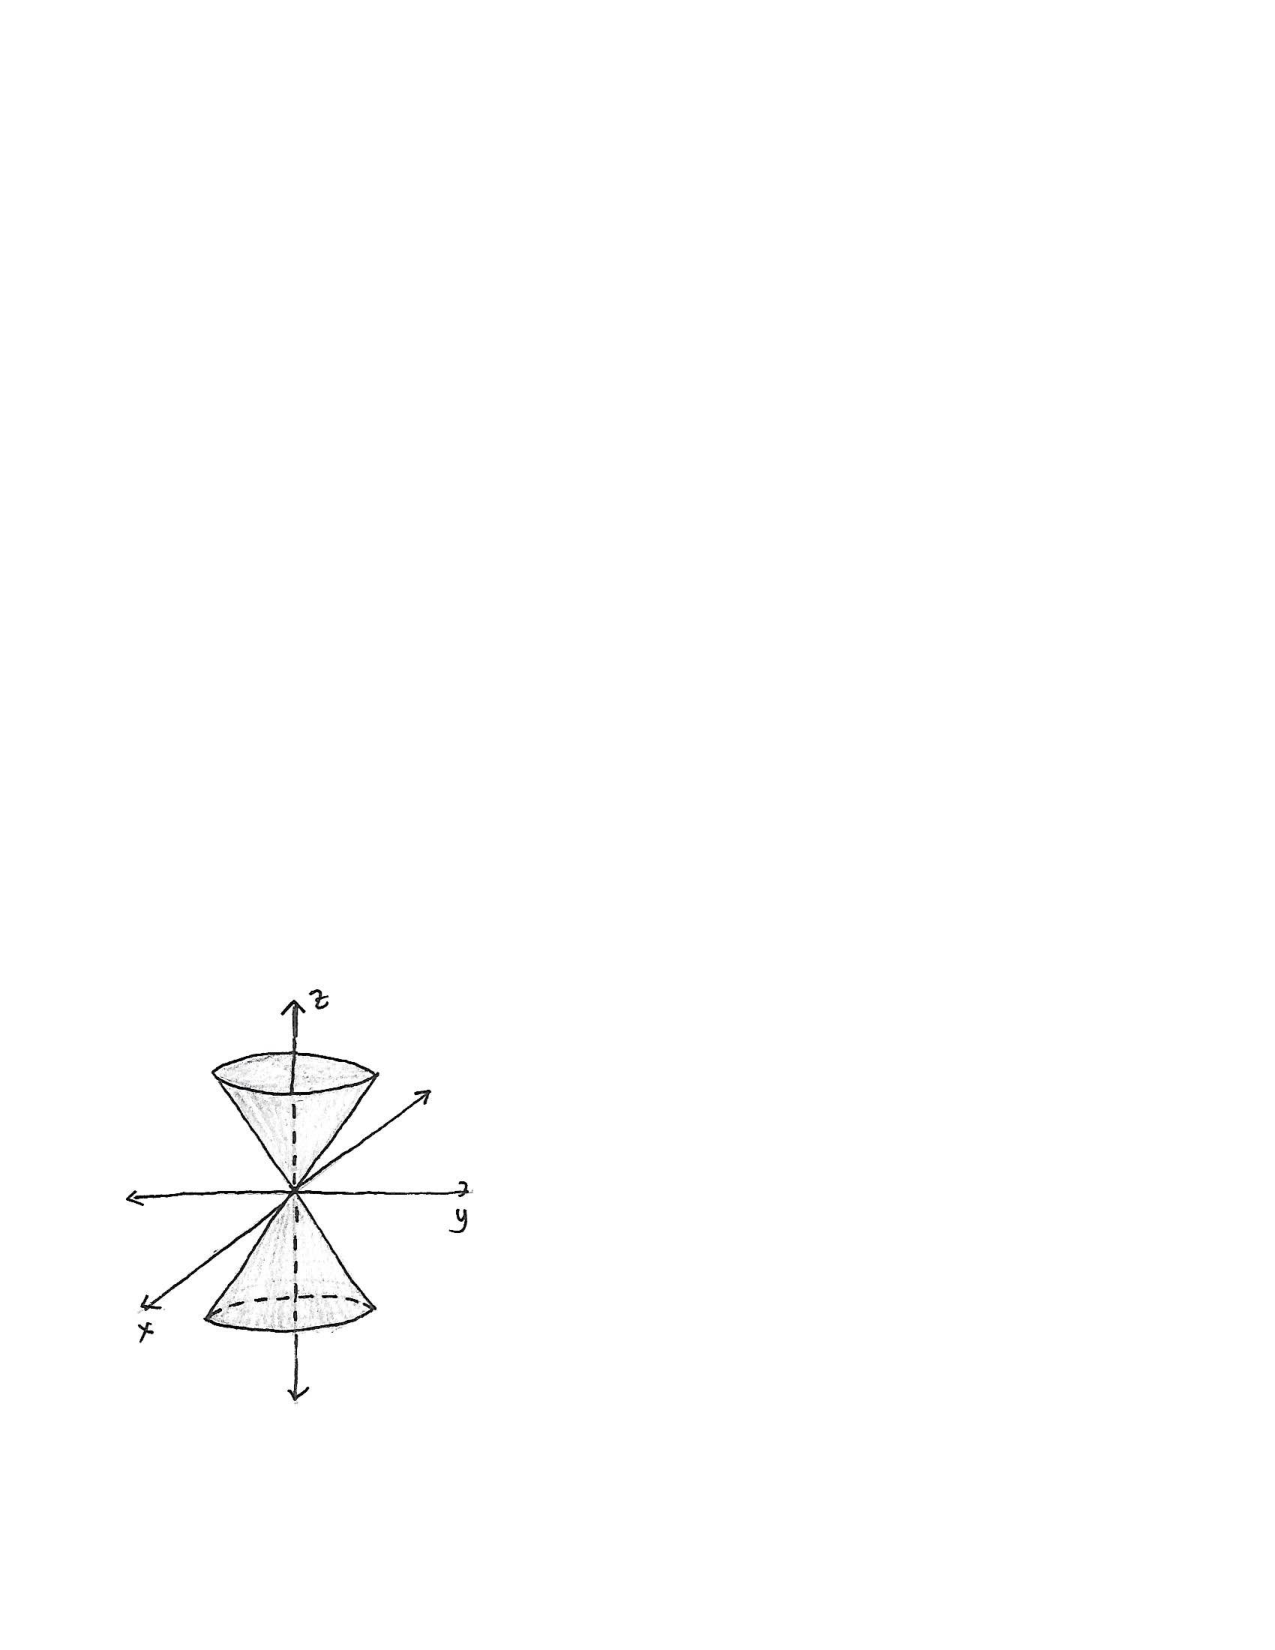
\includegraphics{cone}};
\end{tikzpicture}
\end{image}

Note that if you relax the restriction $\rho\geq 0$, you'll get cone (or double cone) above when $C\neq 0$.

It may seem strange that mathematicians prefer this double cone to the seemingly simpler cones that you're used to. However, it turns out that the double cone is easier to describe algebraically.

You can use the following applet to see what happens when you vary the value of the constant $C$ for each of the constant-coordinate surfaces above:

\href{https://mathinsight.org/spherical_coordinates}{MATH INSIGHT APPLET}

\section{Converting Between Spherical and Cartesian Coordinates}

When converting between spherical coordinates and Cartesian coordinates, it can be useful to use the following equations, which describe the relationship between the two coordinate systems.

\begin{align*}
x &= \rho\cos\theta\sin\phi\\
y &= \rho\sin\theta\sin\phi\\
z &= \rho\cos\phi\\
\rho^2 &= x^2 + y^2 + z^2
\end{align*}

\begin{example}
We'll convert $x^2 + y^2 - z^2 = 1$ from Cartesian coordinates to spherical coordinates. This surface is called an \emph{elliptic hyperboloid}, and its graph is shown below. We'll learn how to identify this and other surfaces later in the course.

\begin{image}
\begin{tikzpicture}
\node[inner sep=0pt] (russell) at (0,0)
    {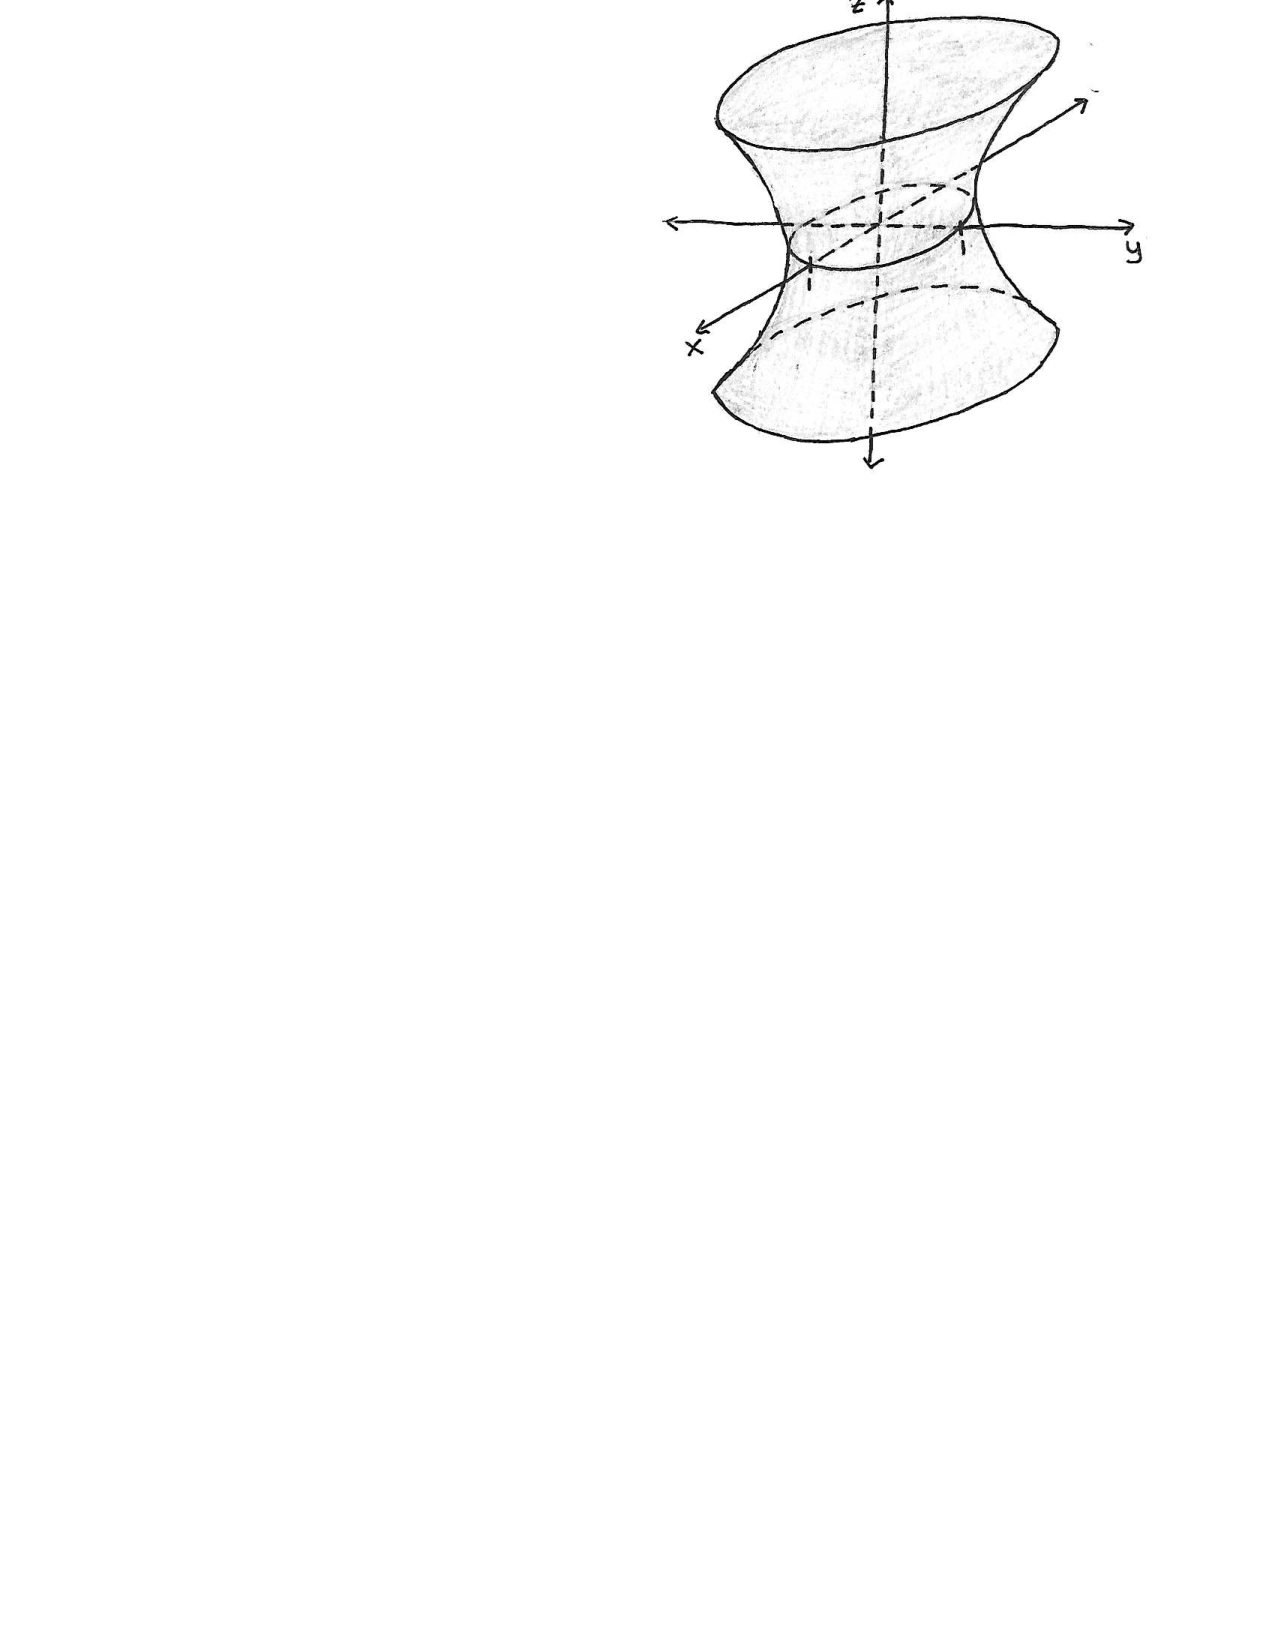
\includegraphics{elliptic_hyper}};
\end{tikzpicture}
\end{image}

Making the substitutions $x = \rho\cos\theta\sin\phi$, $y = \rho\sin\theta\sin\phi$, and $z = \rho\cos\phi$, we have
\[
\rho^2\cos^2\theta\sin^2\phi + \rho^2\sin^2\theta\sin^2\phi - \rho^2\cos^2\phi = 1.
\]
We can factor $\rho^2\sin^2\phi$ out of the first two terms and obtain
\[
\rho^2\sin^2\phi (\cos^2\theta+ \sin^2\theta) - \rho^2\cos^2\phi = 1.
\]
Recalling that $\cos^2\theta+ \sin^2\theta = 1$, we can simplify this to
\[
\rho^2\sin^2\phi  - \rho^2\cos^2\phi = 1.
\]
Recalling the double angle formula $\cos(2\phi) = \cos^2(\phi) - \sin^2(\phi)$, we can simplify this to
\[
\rho^2\cos(2\phi) = 1.
\]
\end{example}

\begin{example}
Sketch the set of points $(\rho,\theta,\phi)$ (in spherical coordinates) such that $0\leq \rho\leq 1$ and $0\leq\phi\leq\pi/4$.

The condition $0\leq \rho\leq 1$ means that we'll have only points within distance $1$ of the origin. The condition $0\leq\phi\leq\pi/4$ means that we'll have only points within angle $\pi/4$ from the $z$-axis. Putting these conditions together, we have the solid ``ice-cream cone'' region sketched below.

\begin{image}
\begin{tikzpicture}
\node[inner sep=0pt] (russell) at (0,0)
    {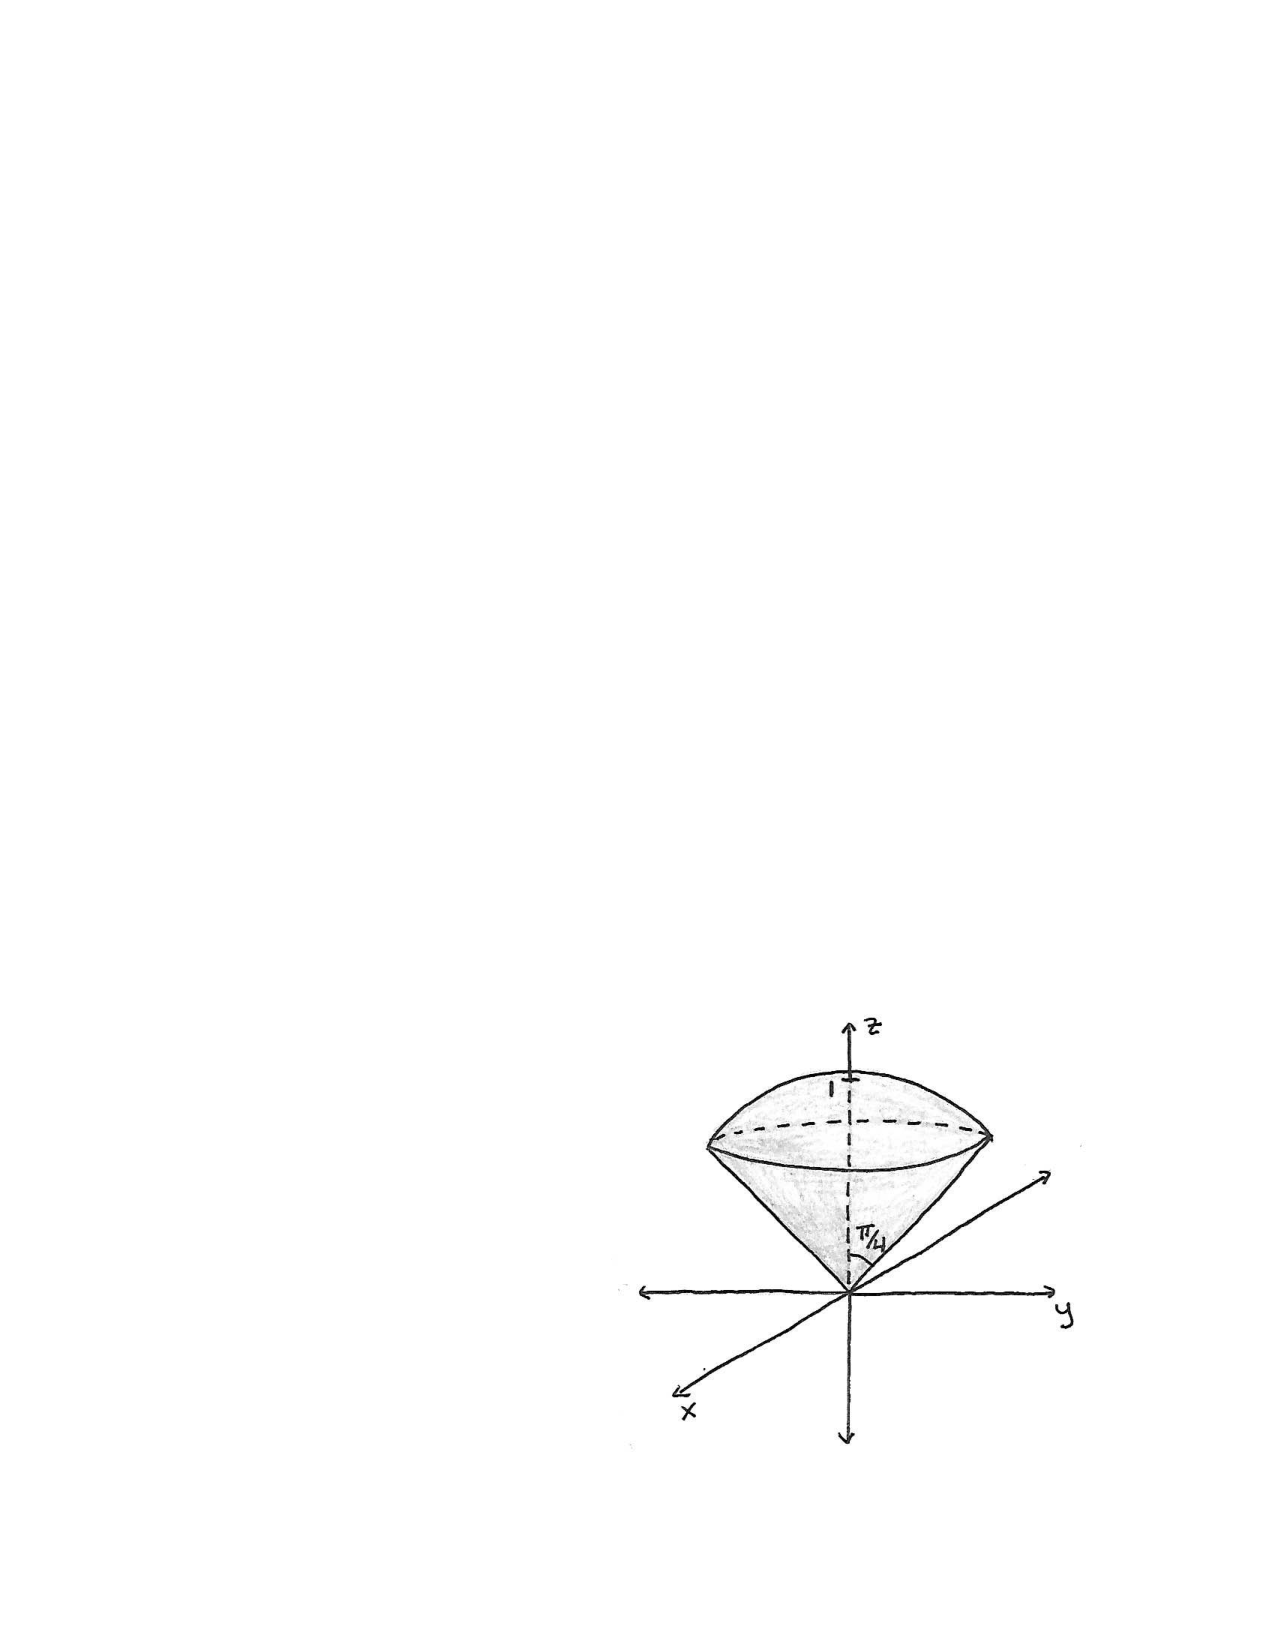
\includegraphics{ice_cream}};
\end{tikzpicture}
\end{image}

\end{example}

\section{Spherical coordinates in $\mathbb{R}^n$ [OPTIONAL]}

Since we've seen polar coordinates in $\mathbb{R}^2$, and cylindrical and spherical coordinates in $\mathbb{R}^3$, you might be wondering if there are similar coordinate systems in $\mathbb{R}^4$, $\mathbb{R}^5$, and so on.

It is possible to define spherical coordinates in $\mathbb{R}^n$ for any $n$, and you can find a description \href{https://en.wikipedia.org/wiki/N-sphere#Spherical_coordinates
}{here}. 

\section{Conclusion}

We introduced spherical coordinates and how to convert between spherical coordinates and Cartesian coordinates, and we discussed the uniqueness of spherical coordinates.

\end{document}